\section{Motivation}

\begin{frame}{Bio AI}
\begin{itemize}
  \item tasks that are easy for people can be very difficult for computers
  \item idea: use algorithms inspired by biological structures and processes
%   \item significant growth in recent years (especially with cheap parallel computing power)
\end{itemize}
\end{frame}

\begin{frame}{Bio AI}
\begin{figure}
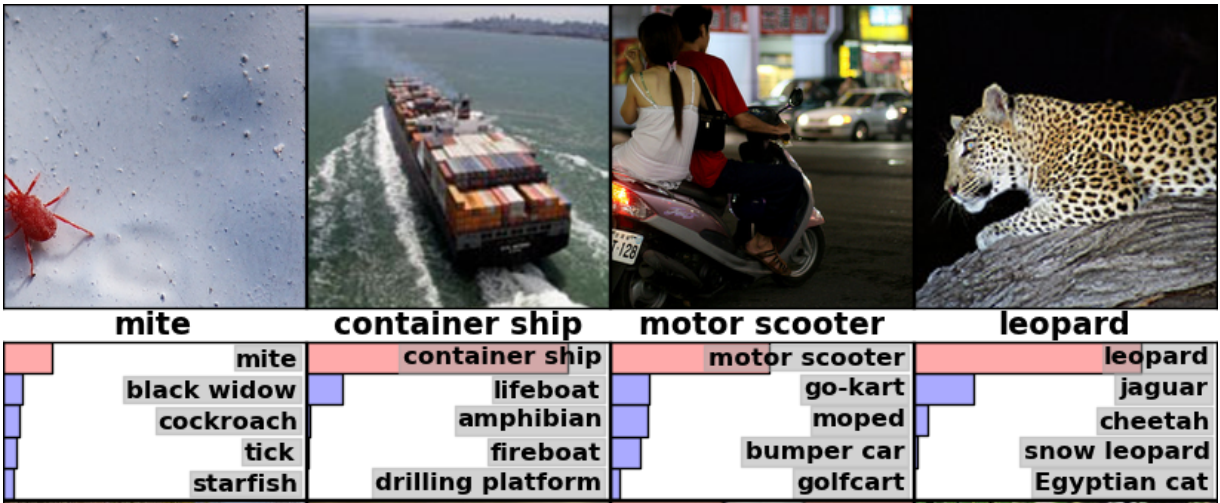
\includegraphics[width=\textwidth]{img/AlexClassification.png}
\captionsetup{singlelinecheck=off,justification=raggedright}
\caption{TensorFlow Image Identification \cite{ImageRecognition}}
\end{figure}
\end{frame}

\begin{frame}{Bio AI}
\begin{figure}
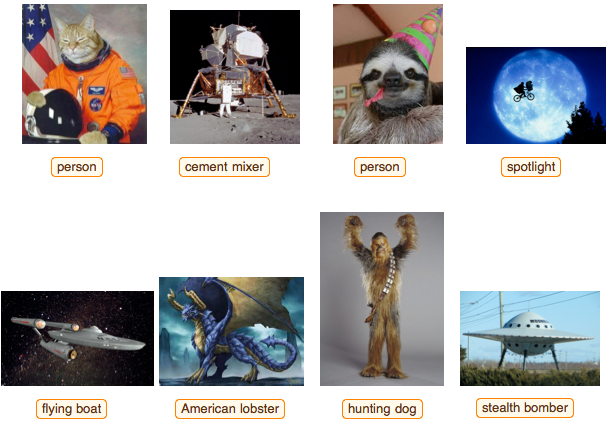
\includegraphics[width=0.8\textwidth]{img/unexpected-images-tested-with-imageidentify.png}
\captionsetup{singlelinecheck=off,justification=raggedright}
\caption{Amusing responses to unexpected images from the Wolfram Image Identification Project \cite{Wolfram2015WolframProject}}
\end{figure}
\end{frame}

\begin{frame}{Bio AI}
\begin{figure}
  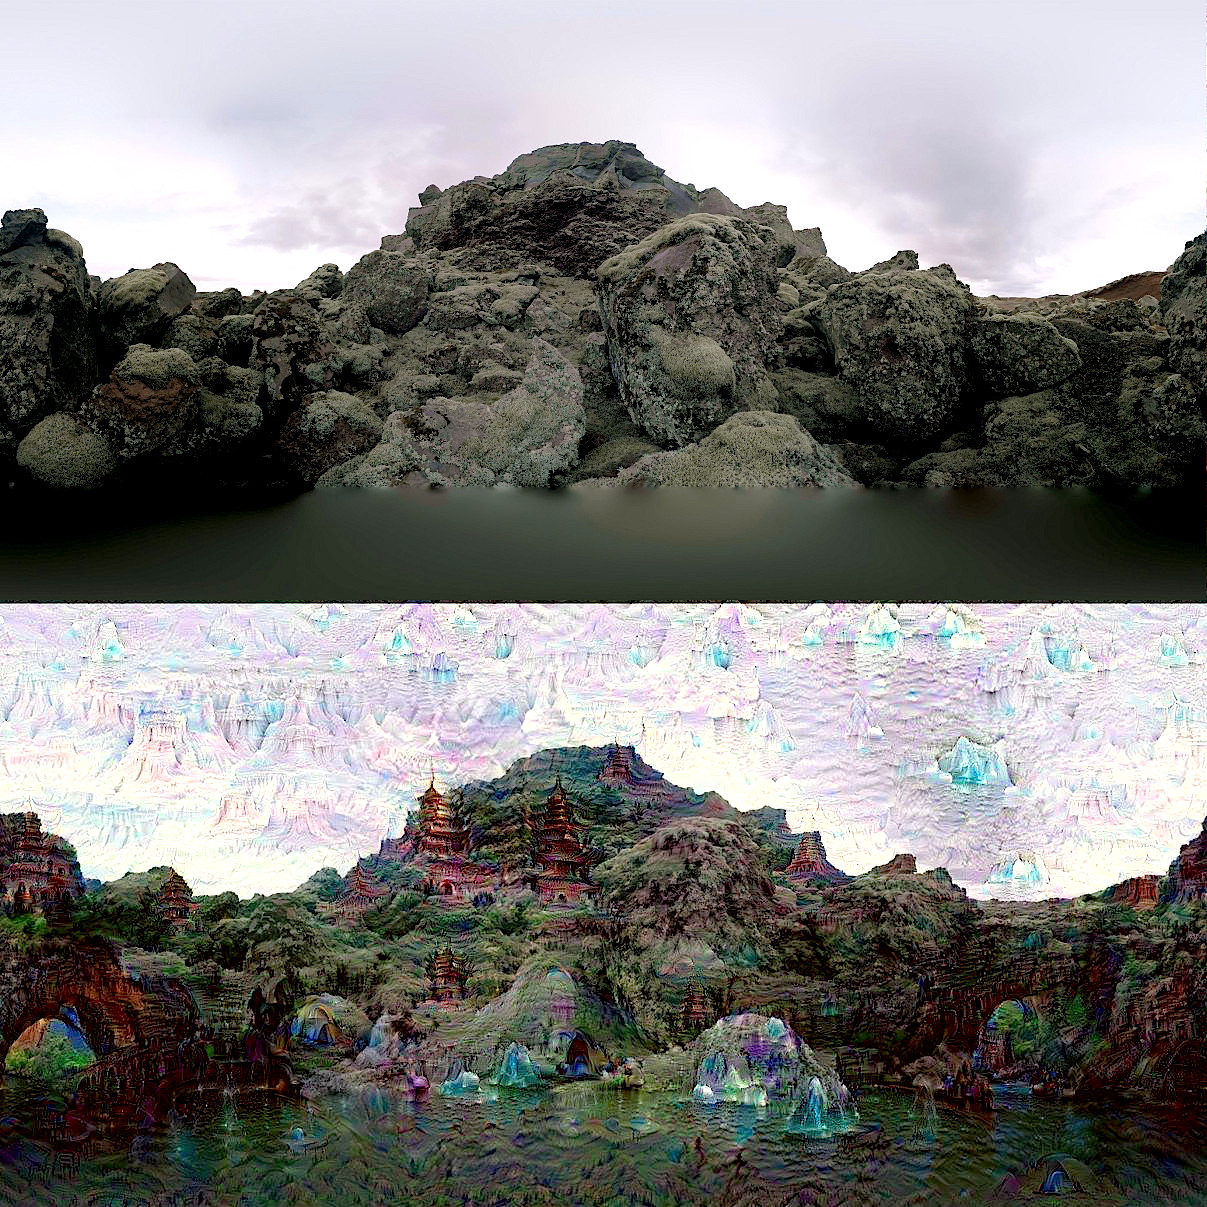
\includegraphics[width=0.6\textwidth]{img/before_after_deepdream}
\captionsetup{singlelinecheck=off,justification=raggedright}
\caption{Google Deep Dream \cite{Mordvintsev2015DeepDreamNetworks}}
\end{figure}
\end{frame}


\begin{frame}{Bio AI}
\begin{figure}
  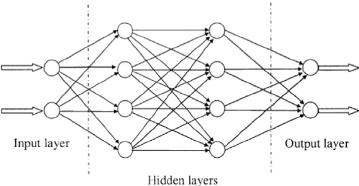
\includegraphics[width=0.8\textwidth]{img/neural_network_schematic}
  \captionsetup{singlelinecheck=off,justification=raggedright}
  \caption{Schematic diagram of an Artificial Neural Network (ANN) \cite[Figure 1]{Ata2015ArtificialReview}}
\end{figure}
\end{frame}

% \begin{frame}{Bio AI}
% shortcomings of backpropagation
% \begin{itemize}
%   \item supervised learning
%   \item no online modification
% \end{itemize}
% \end{frame}

